\documentclass[11pt,a4paper]{article}

%% ── Typography & Encoding ────────────────────────────────────────────────────
\usepackage[margin=1in]{geometry}
\usepackage[T1]{fontenc}
\usepackage[utf8]{inputenc}
\usepackage{lmodern}
\usepackage{microtype}

%% ── Mathematics ──────────────────────────────────────────────────────────────
\usepackage{amsmath,amssymb,bm}

%% ── Tables & Floats ──────────────────────────────────────────────────────────
\usepackage{booktabs}
\usepackage{array}
\usepackage{adjustbox}
\usepackage{multirow}
\usepackage{float}

%% ── Figures ──────────────────────────────────────────────────────────────────
\usepackage{graphicx}
\usepackage{caption}
\usepackage{subcaption}
\usepackage{tikz}
\usetikzlibrary{positioning,arrows.meta,shapes.geometric}

%% ── Color ────────────────────────────────────────────────────────────────────
\usepackage[table]{xcolor}
\definecolor{hustblue}{HTML}{003DA5}
\definecolor{hustbluelight}{HTML}{EBF1FA}
\definecolor{headerblue}{HTML}{E7F0FA}
\definecolor{lightgreen}{HTML}{EAF7EA}
\definecolor{lightyellow}{HTML}{FFF6D8}
\definecolor{lightred}{HTML}{FDEAEA}

%% ── Headers / Footers ────────────────────────────────────────────────────────
\usepackage{fancyhdr}
\pagestyle{fancy}
\fancyhf{}
\fancyhead[L]{\small Modular Representation \& Recognizer Evaluation for ASL Recognition}
\fancyhead[R]{}
\fancyfoot[C]{\small\thepage}
\renewcommand{\headrulewidth}{0.4pt}

%% ── Section Headings ─────────────────────────────────────────────────────────
\usepackage{titlesec}
\titleformat{\section}
  {\large\bfseries\color{hustblue}}
  {\thesection.}{0.6em}{}%
  [\vspace{-5pt}\textcolor{hustblue!60}{\rule{\linewidth}{0.6pt}}]
\titlespacing*{\section}{0pt}{16pt}{8pt}
\titleformat{\subsection}
  {\normalsize\bfseries\color{black}}
  {\thesubsection}{0.5em}{}
\titlespacing*{\subsection}{0pt}{10pt}{4pt}

%% ── Hyperlinks ───────────────────────────────────────────────────────────────
\usepackage{hyperref}
\hypersetup{
  colorlinks  = true,
  linkcolor   = hustblue,
  citecolor   = hustblue,
  urlcolor    = hustblue,
  pdftitle    = {Evaluating Modular Representation and Recognizer Pipelines for ASL Alphabet Recognition},
  pdfauthor   = {Tran Quang Hung, Do Dang Vu, Le Hoang Tung},
}

%% ── Misc ─────────────────────────────────────────────────────────────────────
\usepackage{enumitem}
\setlength{\emergencystretch}{3em}
\setlength{\parskip}{4pt}
\setlength{\parindent}{1em}

\graphicspath{{../report_slides/photos/}}

%% ── Custom Macros ────────────────────────────────────────────────────────────
\newcommand{\codepath}[1]{\texttt{\small #1}}
\newcommand{\pos}[1]{\textcolor{green!55!black}{\textbf{+#1}}}
\newcommand{\neg}[1]{\textcolor{red!60!black}{\textbf{#1}}}

% ─────────────────────────────────────────────────────────────────────────────
\begin{document}
\pagenumbering{Alph}

%% ── Title Page ───────────────────────────────────────────────────────────────
\begin{titlepage}
  \thispagestyle{empty}

  \noindent
  \colorbox{hustblue}{%
    \begin{minipage}{\textwidth}
      \vspace{8pt}
      \centering
      {\color{white}\large\bfseries
        HANOI UNIVERSITY OF SCIENCE AND TECHNOLOGY}\\[3pt]
      {\color{white!80!hustblue}\normalsize
        School of Information and Communication Technology}
      \vspace{8pt}
    \end{minipage}}

  \vspace{2.5cm}
  \begin{center}
    {\Huge\bfseries Computer Vision Capstone Report\par}
    \vspace{0.9cm}
    \textcolor{hustblue}{\rule{0.6\textwidth}{1.2pt}}
    \vspace{0.7cm}

    {\LARGE\bfseries
      Evaluating Modular Representation\\[4pt]
      and Recognizer Pipelines\\[4pt]
      for ASL Alphabet Recognition\par}
    \vspace{0.5cm}
    {\large\itshape
      Does a Smarter Representation Actually Help, or Just Add a New Way to Fail?\par}

    \vspace{1.2cm}
    \textcolor{hustblue}{\rule{0.6\textwidth}{0.6pt}}
    \vspace{1.0cm}

    \begin{tabular}{rl}
      \textbf{Students:}      & Tran Quang Hung -- 20235502 \\[2pt]
                               & Do Dang Vu -- 20235578 \\[2pt]
                               & Le Hoang Tung -- 20235572 \\[6pt]
      \textbf{Topic:}         & Computer Vision -- Sign Language Recognition \\[4pt]
      \textbf{Architecture:}  & Modular Representation $\times$ Recognizer framework \\[4pt]
      \textbf{Backbones:}     & ResNet-18, SigLIP ViT, MLP, SVM, Random Forest \\[4pt]
      \textbf{Dataset:}       & ASL Alphabet (Kaggle) \\
    \end{tabular}

    \vfill
    {\large\today}
  \end{center}
\end{titlepage}

%% ── Front Matter ─────────────────────────────────────────────────────────────
\pagenumbering{roman}
\tableofcontents
\newpage
\pagenumbering{arabic}

%% ═══════════════════════════════════════════════════════════════════════════
\section*{Abstract}
\addcontentsline{toc}{section}{Abstract}
\noindent\colorbox{hustbluelight}{%
  \begin{minipage}{\dimexpr\textwidth-2\fboxsep\relax}
    \vspace{6pt}\small
    This report studies whether "smarter" visual representations actually improve
    static American Sign Language (ASL) alphabet recognition, or merely add
    complexity and new failure modes. We build a modular framework that decouples
    a \emph{Representation} module (raw image, MediaPipe hand-crop, MediaPipe
    landmarks, or image enhancement) from a \emph{Recognizer} module (ResNet-18,
    a pretrained SigLIP Vision Transformer, or a landmark classifier --- MLP, SVM,
    or Random Forest), yielding 13 distinct, independently evaluable pipelines.
    %
    Beyond clean-image accuracy, we evaluate macro-F1, robustness under eight
    image corruptions, and a previously-hidden metric --- the fraction of images
    for which the upstream hand detector fails and is silently excluded from the
    standard accuracy computation. We further use Grad-CAM and UMAP/t-SNE
    projections of the recognizer's feature space to inspect \emph{why} pipelines
    succeed or fail, not just by how much.
    %
    The results show that pipelines built on MediaPipe hand detection report
    competitive clean accuracy (up to 98.5\%) yet collapse to 0\% accuracy under
    the worst image corruption, and that the true end-to-end accuracy of the best
    such pipeline is 81.15\%, not the 98.5\% it reports --- a 17-point gap hidden
    by the standard metric. Simpler pipelines that skip hand detection entirely
    (raw image or lightweight enhancement, fed directly to ResNet-18 or SigLIP)
    never drop below 70\% accuracy under any corruption, showing that architectural
    simplicity can be a robustness advantage, not just a baseline.
    \vspace{6pt}
  \end{minipage}}
\vspace{1em}

%% ═══════════════════════════════════════════════════════════════════════════
\section{Introduction}

\subsection{Why Automatic Sign Language Recognition Matters}
\label{sec:motivation}

American Sign Language (ASL) is the primary language of an estimated half a
million to two million Deaf and hard-of-hearing people in North America, and
manual fingerspelling of the alphabet is used whenever a signer needs to
produce a word that has no dedicated sign --- names, addresses, technical terms,
or borrowed vocabulary. The communication gap this creates is not abstract: a
Deaf person interacting with a hearing person who does not know ASL has no
shared channel, and the burden of bridging that gap --- hiring an interpreter,
exchanging written notes, or relying on lip-reading --- falls disproportionately
on the Deaf individual. Figure~\ref{fig:motivation_diagram} summarizes the
causal chain from this communication gap to the system studied in this report.

\begin{figure}[H]
  \centering
  \resizebox{\textwidth}{!}{%
  \begin{tikzpicture}[
      node distance=10mm and 10mm,
      box/.style={draw, rounded corners, fill=hustbluelight, align=center,
                  minimum height=1.5cm, minimum width=3.6cm, font=\normalsize,
                  text width=3.3cm, inner sep=6pt, drop shadow},
      problembox/.style={box, fill=lightred},
      solutionbox/.style={box, fill=lightgreen},
      arrow/.style={-{Stealth[length=3mm]}, thick, hustblue, line width=1pt}
    ]
    % Top row: the problem
    \node[problembox] (gap) {Communication gap between Deaf/HoH signers and non-signing hearing people};
    \node[box, right=of gap] (asl) {ASL is their shared language; fingerspelling covers words with no dedicated sign};
    \node[problembox, right=of asl] (barrier) {Few hearing people read ASL fluently $\Rightarrow$ the barrier persists in daily life};

    % Bottom row: the solution, aligned under the top row
    \node[solutionbox, below=of gap] (impact) {Enables real-time captioning, assistive learning tools, accessible HCI};
    \node[box, below=of asl] (input) {Webcam frame $\rightarrow$ Representation $\rightarrow$ Recognizer $\rightarrow$ A--Z label};
    \node[solutionbox, below=of barrier] (system) {Automatic ASL alphabet recognition system (this report)};

    \draw[arrow] (gap) -- (asl);
    \draw[arrow] (asl) -- (barrier);
    \draw[arrow] (barrier) -- (system);
    \draw[arrow] (system) -- (input);
    \draw[arrow] (input) -- (impact);
  \end{tikzpicture}}
  \caption{Motivation chain: a persistent communication gap (top row) motivates
    automatic ASL recognition; the system itself is the pipeline studied in
    this report (Section~\ref{sec:framework}, bottom row, read right to left);
    its purpose is to enable downstream accessibility applications that do not
    require specialized hardware.}
  \label{fig:motivation_diagram}
\end{figure}

Building such a system only requires a standard webcam, which makes it
substantially cheaper to deploy than dedicated sign-language gloves or
depth-sensing hardware. The remaining question is purely a computer vision
one: \emph{which combination of preprocessing and classification produces a
system that is accurate, robust, and fast enough to be useful} --- and that
question turns out to be far less settled than it first appears, because the
intuitive idea that ``adding a hand detector should help'' is often false in
practice, as Section~\ref{sec:case_study} demonstrates directly.

\subsection{Project Motivation: Does a Smarter Representation Help?}

A static ASL alphabet recognizer is conventionally built as a two-stage
pipeline: a \emph{representation} stage that turns a raw webcam frame into
something more tractable (e.g., a hand crop or hand-pose landmarks), followed
by a \emph{recognizer} stage that turns that representation into one of 26
letter labels. The representation stage is usually treated as an unambiguous
improvement --- cropping the hand removes background clutter, and landmarks
remove skin-tone and lighting variation entirely. This project tests that
assumption directly, asking:

\begin{itemize}[leftmargin=1.4em]
  \item Does hand-cropping or landmark extraction actually improve recognition
        accuracy, or does it just add an additional component that can fail?
  \item Is a pretrained Vision Transformer worth its extra latency over a
        small, fine-tuned CNN?
  \item Does the standard way of reporting accuracy correctly reflect how the
        system would behave in real, uncontrolled use?
  \item Which pipeline is actually the best choice once accuracy,
        robustness, and speed are all considered together?
\end{itemize}

\subsection{Report Scope}

This report covers a single dataset (the Kaggle ASL Alphabet dataset, 26
static A--Z classes) and 13 distinct representation/recognizer combinations,
evaluated under one shared protocol: clean accuracy, macro-F1, robustness
under eight corruption types, latency, and (for MediaPipe-based pipelines)
hand-detection failure rate. Continuous, motion-based signs (e.g., J and Z in
real ASL) are treated as static targets, consistent with the rest of the
literature on static fingerspelling recognition.

\subsection{Main Contributions of This Report}

\begin{enumerate}[leftmargin=1.6em]
  \item A modular framework that decouples representation and recognizer
        choices, enabling 13 pipelines to be compared under one protocol
        instead of 13 separate, inconsistent setups.
  \item An evaluation protocol that exposes a metric pitfall hidden in the
        common practice of excluding ``no hand detected'' frames from the
        accuracy denominator (Section~\ref{sec:metrics}).
  \item A robustness benchmark across eight corruption types that
        differentiates pipelines that look identical on clean data.
  \item Qualitative tooling --- step-by-step visual grids, Grad-CAM, and
        UMAP/t-SNE projections of the recognizer's feature space --- that
        explains \emph{why}, not just \emph{whether}, a pipeline fails.
  \item A concrete case study quantifying the gap between reported and real
        accuracy for the best-looking MediaPipe-based pipeline.
\end{enumerate}

%% ═══════════════════════════════════════════════════════════════════════════
\section{Problem Formulation}
\label{sec:framework}

Let $x \in \mathcal{X}$ be an RGB webcam frame and $y \in \mathcal{Y} =
\{A, \dots, Z\}$ its ground-truth label. We decompose the recognition system
into two independently swappable modules:
\begin{equation}
  \hat{y} = R\big(\,\Phi(x)\,\big),
\end{equation}
where $\Phi: \mathcal{X} \rightarrow \mathcal{Z}$ is the \emph{representation
function} and $R: \mathcal{Z} \rightarrow \mathcal{Y} \cup \{\textsc{Unknown}\}$
is the \emph{recognizer}. Critically, $\Phi$ is \emph{partial}: for
MediaPipe-based representations, $\Phi(x)$ is undefined (returns $\varnothing$)
whenever the upstream hand detector fails to locate a hand in $x$, in which
case $R$ trivially outputs \textsc{Unknown} without ever running its
classification logic. This single design fact is the source of the central
finding of this report (Section~\ref{sec:case_study}): a pipeline's measured
accuracy depends entirely on how images with $\Phi(x) = \varnothing$ are
counted, and the conventional choice (excluding them) systematically
overstates real-world performance.

A pipeline is therefore fully specified by the pair $(\Phi, R)$. We study
4 representation functions and 5 recognizers (Section~\ref{sec:methods}),
yielding 13 type-compatible $(\Phi, R)$ combinations (image-typed
representations pair with image-based recognizers; the landmark
representation pairs with landmark-based recognizers).

%% ═══════════════════════════════════════════════════════════════════════════
\section{Proposed Framework}
\label{sec:methods}

\subsection{Two-Module Architecture}

Figure~\ref{fig:repr_grid} previews the four representation functions studied,
applied to the same five test images; Table~\ref{tab:recognizers} lists the
five recognizers. Any image-typed representation can be paired with any
image-based recognizer, and the landmark representation pairs with any of the
three landmark-based recognizers, for $4\times2 + 1\times3 = 11$ structurally
distinct combinations; counting the two enhancement variants (CLAHE, Gamma)
each paired with both image recognizers brings the evaluated set to 13
pipelines in total (Table~\ref{tab:summary_results}).

\subsection{Representation Functions}

\begin{itemize}[leftmargin=1.4em]
  \item \textbf{Raw image:} resize to $224\times224$; no other processing.
  \item \textbf{MediaPipe Crop:} MediaPipe HandLandmarker locates 21 hand
        keypoints, from which a bounding box is computed; the frame is cropped
        to that box (with a fixed pixel padding) and resized.
  \item \textbf{MediaPipe Landmarks:} the same 21 keypoints are kept as raw
        coordinates and converted into a 42-dimensional feature vector,
        normalized relative to the wrist keypoint and scaled by the maximum
        absolute coordinate value:
        \begin{equation}
          \tilde{p}_i = p_i - p_{\text{wrist}}, \qquad
          f_i = \frac{\tilde{p}_i}{\max_j |\tilde{p}_j|}, \qquad i = 1, \dots, 21,
          \label{eq:landmark_norm}
        \end{equation}
        producing $f \in \mathbb{R}^{42}$ (concatenated $x,y$ per point) that
        is invariant to translation and scale but discards all texture and
        skin-color information.
  \item \textbf{Enhancement:} CLAHE, gamma correction, unsharp-mask
        sharpening, or non-local-means denoising applied to the raw image
        before resizing, used to test whether photometric preprocessing
        (rather than spatial cropping) helps.
\end{itemize}

\begin{figure}[H]
  \centering
  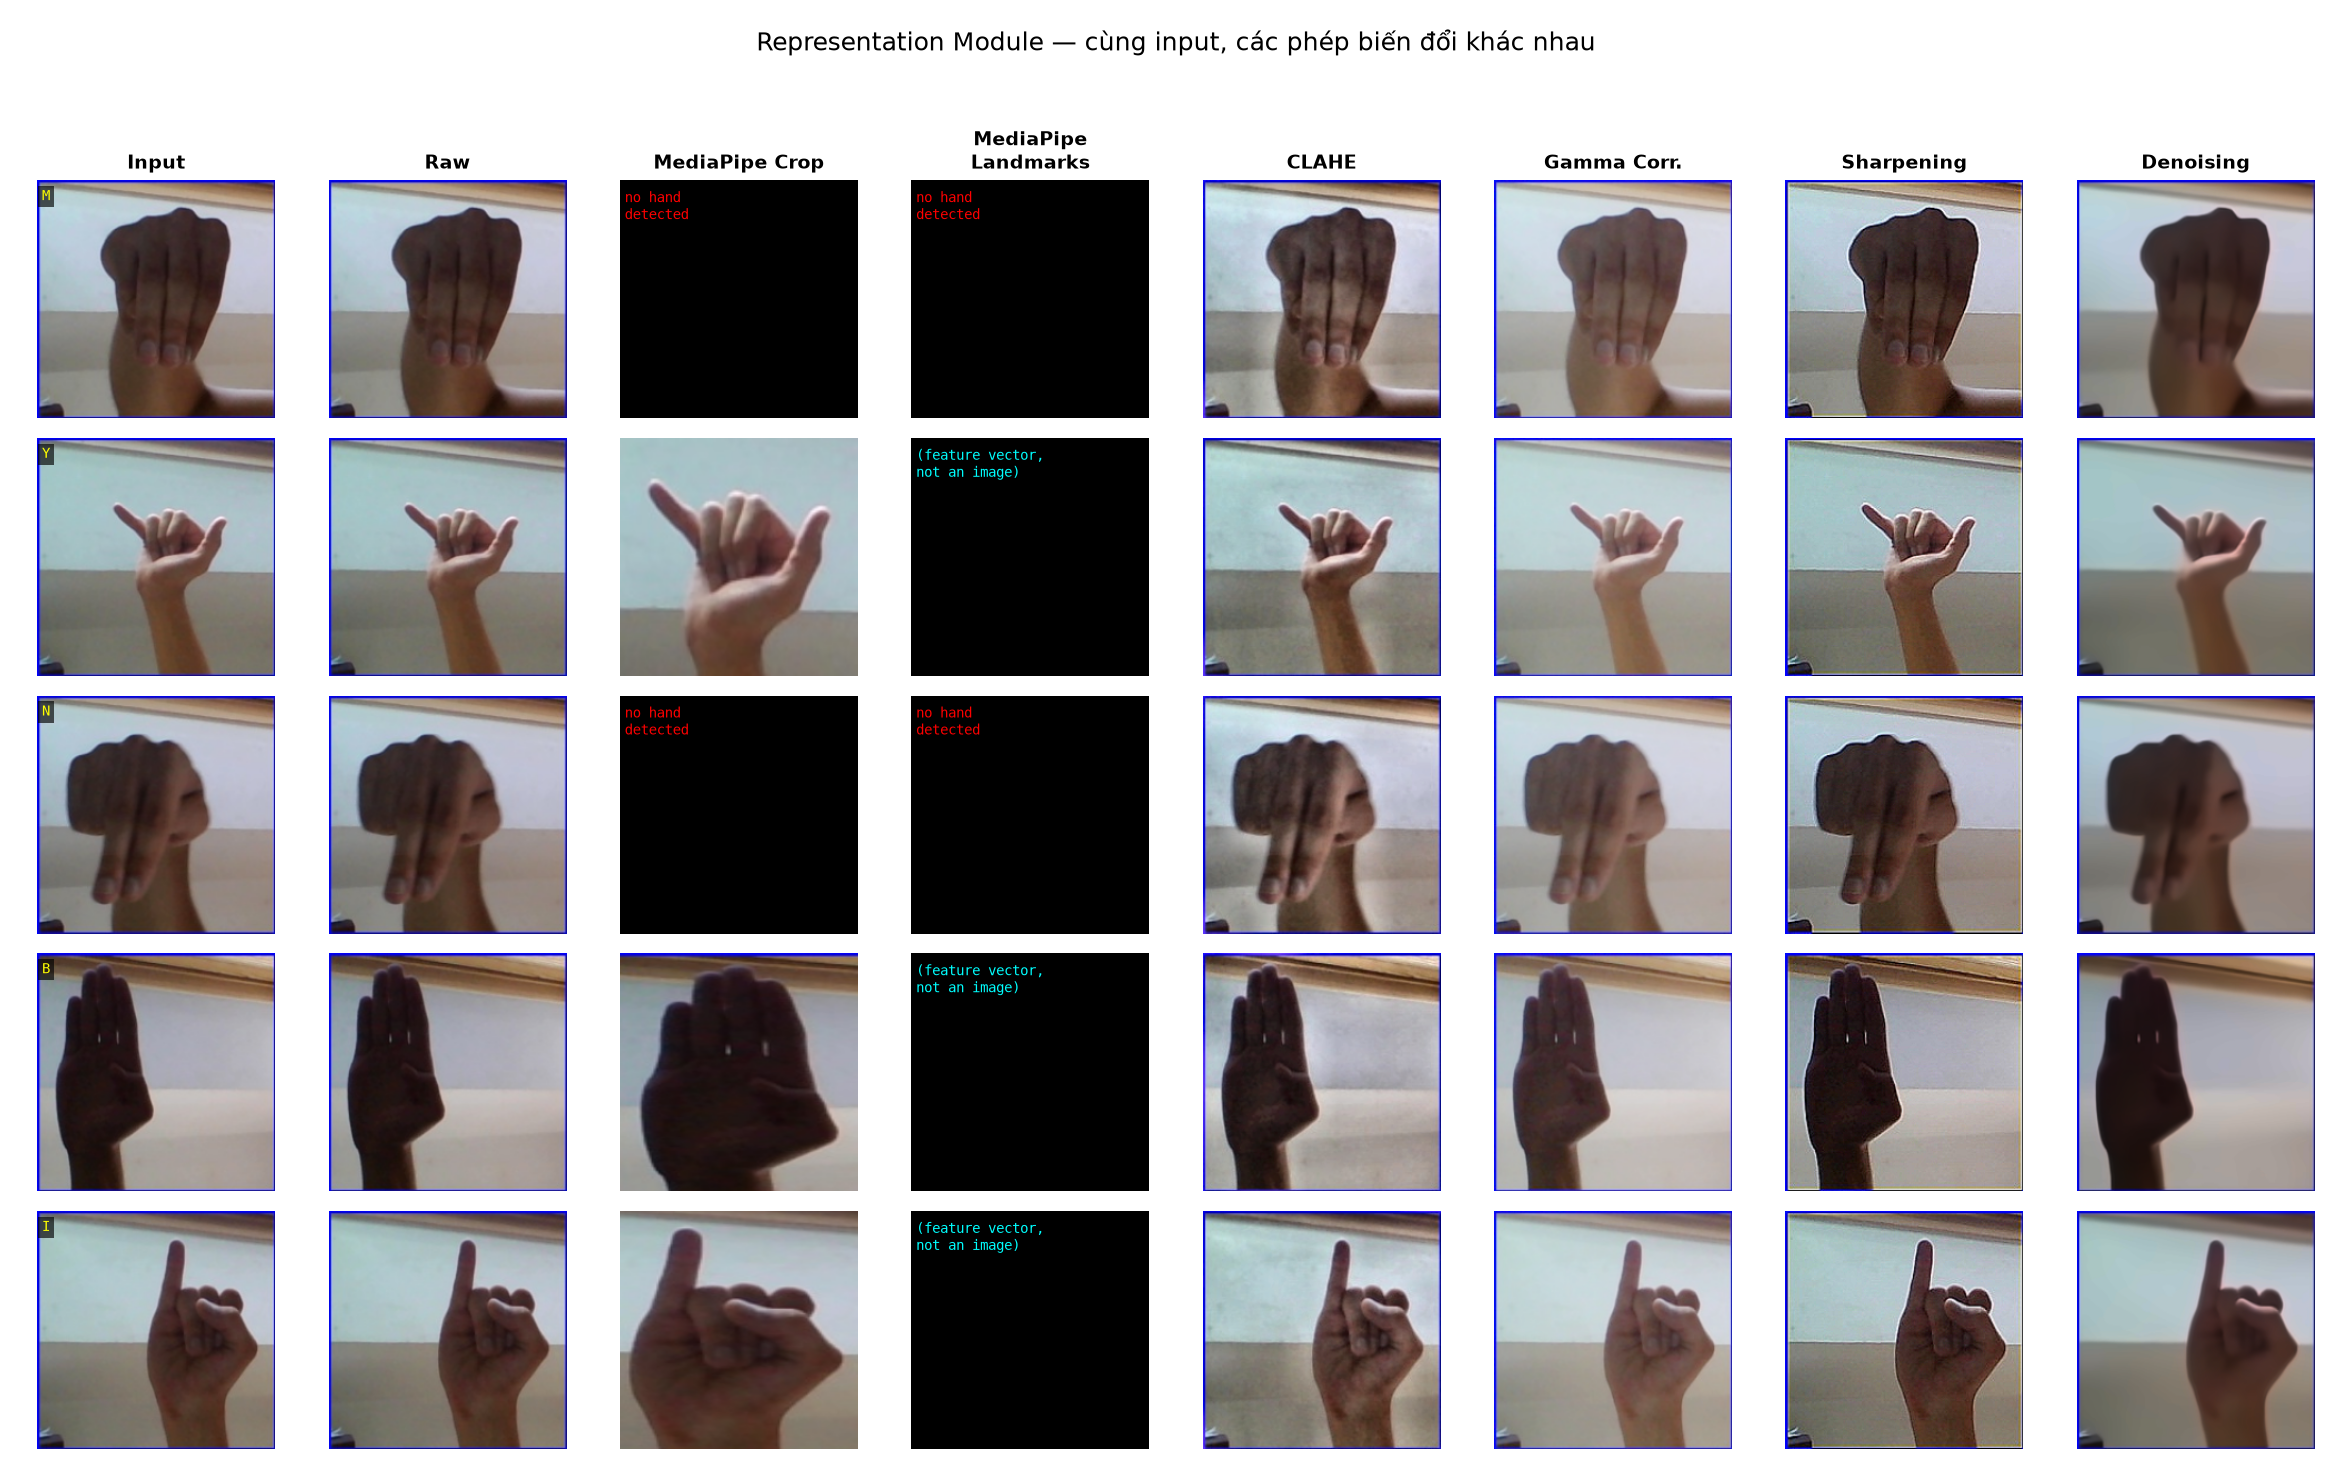
\includegraphics[width=0.92\textwidth]{grid_representation.png}
  \caption{Five sample test images (rows) through six concrete representation
    instances (columns): Raw, MediaPipe Crop, CLAHE, Gamma, Sharpening,
    Denoising. The MediaPipe Crop column is black on 3 of 5 rows --- the hand
    detector failed on those (low-contrast) images, illustrating the partial
    nature of $\Phi$ described in Section~\ref{sec:framework}.}
  \label{fig:repr_grid}
\end{figure}

\subsection{Recognizers}

\begin{table}[H]
\centering
\caption{Recognizer modules and their expected input type.}
\label{tab:recognizers}
\small
\begin{adjustbox}{max width=\textwidth}
\begin{tabular}{lll}
\toprule
\rowcolor{headerblue}
Recognizer & Model family & Input \\
\midrule
ResNet-18 (\codepath{resnet18\_asl} / \codepath{torchvision\_classifier}) & CNN, fine-tuned on ASL & $224\times224$ image \\
SigLIP ViT (HuggingFace) & Vision Transformer, pretrained & $224\times224$ image \\
Landmark MLP & Multi-layer perceptron & 42-d vector \\
Landmark SVM & Support Vector Machine & 42-d vector \\
Landmark RF & Random Forest & 42-d vector \\
\bottomrule
\end{tabular}
\end{adjustbox}
\end{table}

The pretrained ViT recognizer is the strongest model in isolation; the
landmark-based classifiers are the lightest and fastest (Table~\ref{tab:summary_results}).
The central question of this report is whether pairing a strong recognizer
with a hand-cropping representation actually compounds into a better
\emph{system}, or whether the representation stage's own failure rate
cancels out the recognizer's quality gain.

%% ═══════════════════════════════════════════════════════════════════════════
\section{Evaluation Protocol}
\label{sec:metrics}

\subsection{The Hidden Accuracy Pitfall}

The implementation's standard accuracy metric is computed only over the
subset of test images for which the representation successfully produced an
output:
\begin{equation}
  \text{clean\_accuracy} =
  \frac{\#\{i : \hat{y}_i = y_i \,\wedge\, \Phi(x_i) \neq \varnothing\}}
       {\#\{i : \Phi(x_i) \neq \varnothing\}}.
  \label{eq:clean_acc}
\end{equation}
Images with $\Phi(x_i) = \varnothing$ (no hand detected) are removed from
\emph{both} the numerator and the denominator, rather than counted as
incorrect. We additionally compute the metric that matches how a deployed
system would actually be judged by a user:
\begin{equation}
  \text{real\_accuracy} =
  \frac{\#\{i : \hat{y}_i = y_i\}}
       {\#\{i : 1 \le i \le N\}},
  \qquad \text{where } \hat{y}_i = \textsc{Unknown} \text{ counts as incorrect.}
  \label{eq:real_acc}
\end{equation}
We also report the \emph{hand-detection failure rate},
$\text{HDFR} = \#\{i : \Phi(x_i) = \varnothing\} / N$, which applies only to
MediaPipe-based representations (it is identically zero for Raw and
Enhancement, since those representations never fail to produce an output).
Section~\ref{sec:case_study} shows that the gap between
Eq.~\eqref{eq:clean_acc} and Eq.~\eqref{eq:real_acc} can exceed 17 percentage
points for a pipeline with a high HDFR.

\subsection{Robustness Benchmark}

To test behavior beyond the (visually clean, studio-lit) test set, every
pipeline is re-evaluated on eight corrupted variants of the test set:
low-light, overexposure, motion blur, Gaussian noise, rotation, scale shift,
partial occlusion, and crop shift. We report the worst single-corruption
accuracy (the pipeline's failure ceiling) and the average accuracy drop
relative to clean accuracy.

%% ═══════════════════════════════════════════════════════════════════════════
\section{Experimental Setup}

\subsection{Dataset}

We use the Kaggle ASL Alphabet dataset~\cite{aslalphabet}: 26 static A--Z
classes, photographed under relatively uniform studio lighting against a
fairly clean background. The training split ($\sim$78{,}000 images) is used to
fine-tune ResNet-18 and to train the landmark MLP/SVM/RF classifiers; the
\codepath{test\_split} subset (2{,}600 images, 100 per class) is held out for
all clean-accuracy and robustness evaluation reported in this paper. The ViT
recognizer uses third-party pretrained weights and is not further fine-tuned
on this dataset.

\begin{figure}[H]
  \centering
  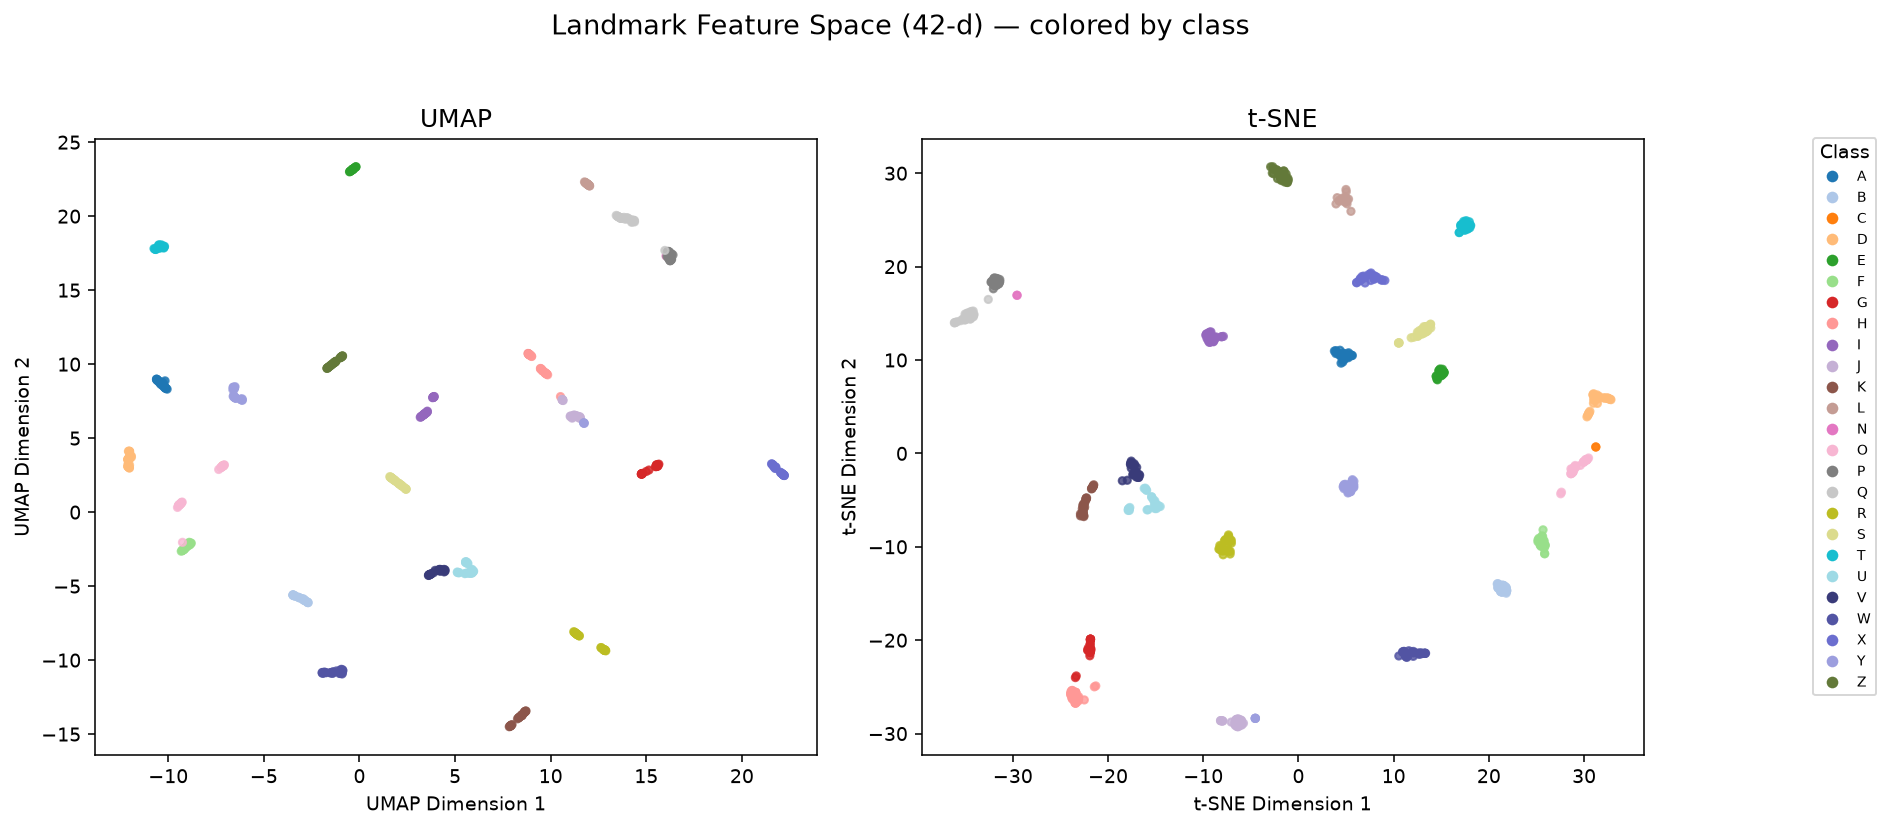
\includegraphics[width=0.62\textwidth]{embedding_landmarks_by_class.png}
  \caption{UMAP (left) and t-SNE (right) projection of the 42-dimensional
    MediaPipe landmark vectors (Eq.~\ref{eq:landmark_norm}), 30 images per
    class sampled from \codepath{test\_split}, colored by ground-truth class.
    All 26 classes form well-separated, compact clusters purely from hand
    pose --- the dataset is intrinsically easy to classify when the hand is
    successfully detected, which is exactly why clean accuracy alone fails to
    distinguish pipeline quality (Section~\ref{sec:case_study}): nearly every
    pipeline that sees the hand classifies it correctly.}
  \label{fig:embedding_landmarks}
\end{figure}

\subsection{Why Clean Accuracy Alone Is Insufficient}

The dataset's studio conditions, combined with the clean class separability
shown in Figure~\ref{fig:embedding_landmarks}, mean that most pipelines reach
99--100\% clean accuracy (Table~\ref{tab:summary_results}). This is precisely
the scenario the robustness benchmark is designed for: when nearly every
pipeline looks equally good on clean data, only stress-testing under
corruption and auditing the accuracy formula itself (Section~\ref{sec:metrics})
reveal meaningful differences.

%% ═══════════════════════════════════════════════════════════════════════════
\section{Quantitative Results}

Table~\ref{tab:summary_results} reports clean accuracy, macro-F1, worst-case
corruption accuracy, hand-detection failure rate, and inference speed for all
13 pipelines, sorted by clean accuracy.

\begin{table}[H]
\centering
\caption{Full results across 13 pipelines on the ASL Alphabet \codepath{test\_split}.
  Bold rows are referenced directly in Section~\ref{sec:case_study}.}
\label{tab:summary_results}
\small
\begin{adjustbox}{max width=\textwidth}
\begin{tabular}{lrrrrr}
\toprule
\rowcolor{headerblue}
Pipeline & Clean Acc. & Macro-F1 & Worst-case & Hand-fail & FPS \\
\midrule
raw\_siglip                    & 1.0000 & 1.0000 & 0.8912 & 0.0\%   & 6.3   \\
enhancement\_gamma\_vit         & 1.0000 & 1.0000 & 0.8927 & 0.0\%   & 22.9  \\
enhancement\_clahe\_vit         & 0.9996 & 0.9996 & 0.8629 & 0.0\%   & 9.3   \\
raw\_resnet18                  & 0.9985 & 0.9985 & 0.9202 & 0.0\%   & 222.3 \\
enhancement\_gamma\_resnet18    & 0.9985 & 0.9985 & 0.9135 & 0.0\%   & 21.8  \\
enhancement\_sharpen\_resnet18  & 0.9965 & 0.9965 & \neg{0.1010} & 0.0\%   & 244.6 \\
enhancement\_clahe\_resnet18    & 0.9954 & 0.9954 & 0.7356 & 0.0\%   & 16.7  \\
enhancement\_denoise\_resnet18  & 0.9954 & 0.9954 & 0.7012 & 0.0\%   & 7.9   \\
\rowcolor{lightred}
\textbf{mediapipe\_crop\_vit}   & \textbf{0.9851} & 0.9707 & \neg{0.0000} & \textbf{17.15\%} & 11.2  \\
mediapipe\_landmarks\_rf       & 0.9741 & 0.9552 & \neg{0.0000} & 17.15\% & 16.6  \\
mediapipe\_landmarks\_svm      & 0.9706 & 0.9723 & \neg{0.0000} & 17.15\% & 19.8  \\
mediapipe\_landmarks\_mlp      & 0.9705 & 0.9556 & \neg{0.0000} & 17.15\% & 35.0  \\
\rowcolor{lightred}
\textbf{mediapipe\_crop\_resnet18} & \textbf{0.8859} & 0.8627 & \neg{0.0000} & \textbf{17.15\%} & 18.9  \\
\bottomrule
\end{tabular}
\end{adjustbox}
\end{table}

Three patterns are immediately visible. First, every pipeline that skips hand
detection entirely (Raw or Enhancement representations) reaches at least
99.5\% clean accuracy and never drops below 70\% worst-case accuracy. Second,
every pipeline built on MediaPipe (crop or landmarks) drops to exactly
\neg{0.0000} worst-case accuracy, regardless of how strong its recognizer is
--- the SigLIP-based \codepath{mediapipe\_crop\_vit} collapses just as
completely as the much weaker \codepath{mediapipe\_crop\_resnet18}. Third, the
17.15\% hand-detection failure rate is identical across all five
MediaPipe-based pipelines, since it is a property of the shared representation
stage, not of the recognizer.

\begin{figure}[H]
  \centering
  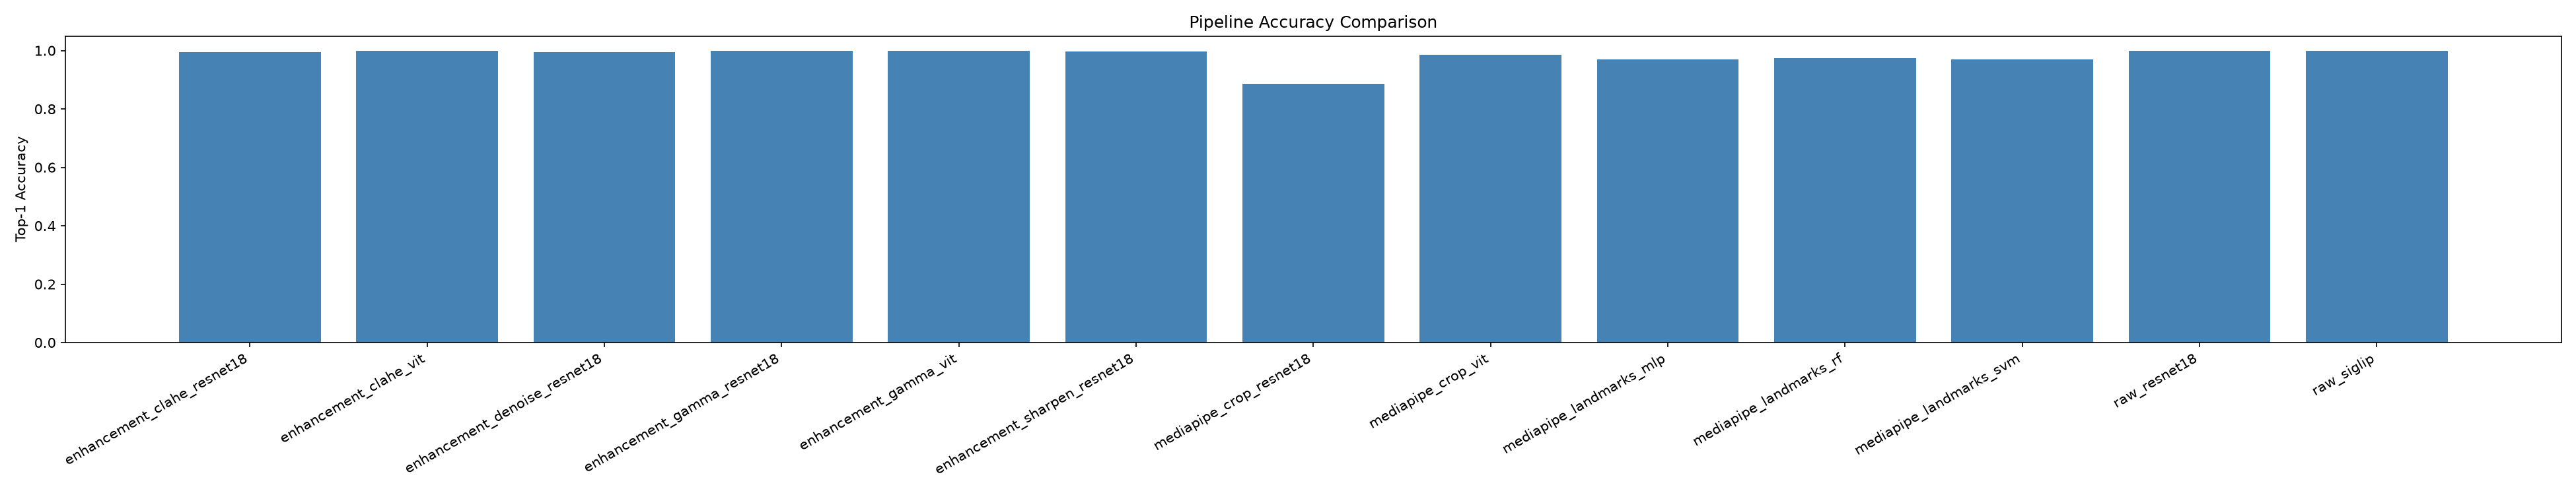
\includegraphics[width=0.85\textwidth]{pipeline_accuracy_comparison.png}
  \caption{Clean accuracy across all 13 pipelines.}
  \label{fig:acc_chart}
\end{figure}

\begin{figure}[H]
  \centering
  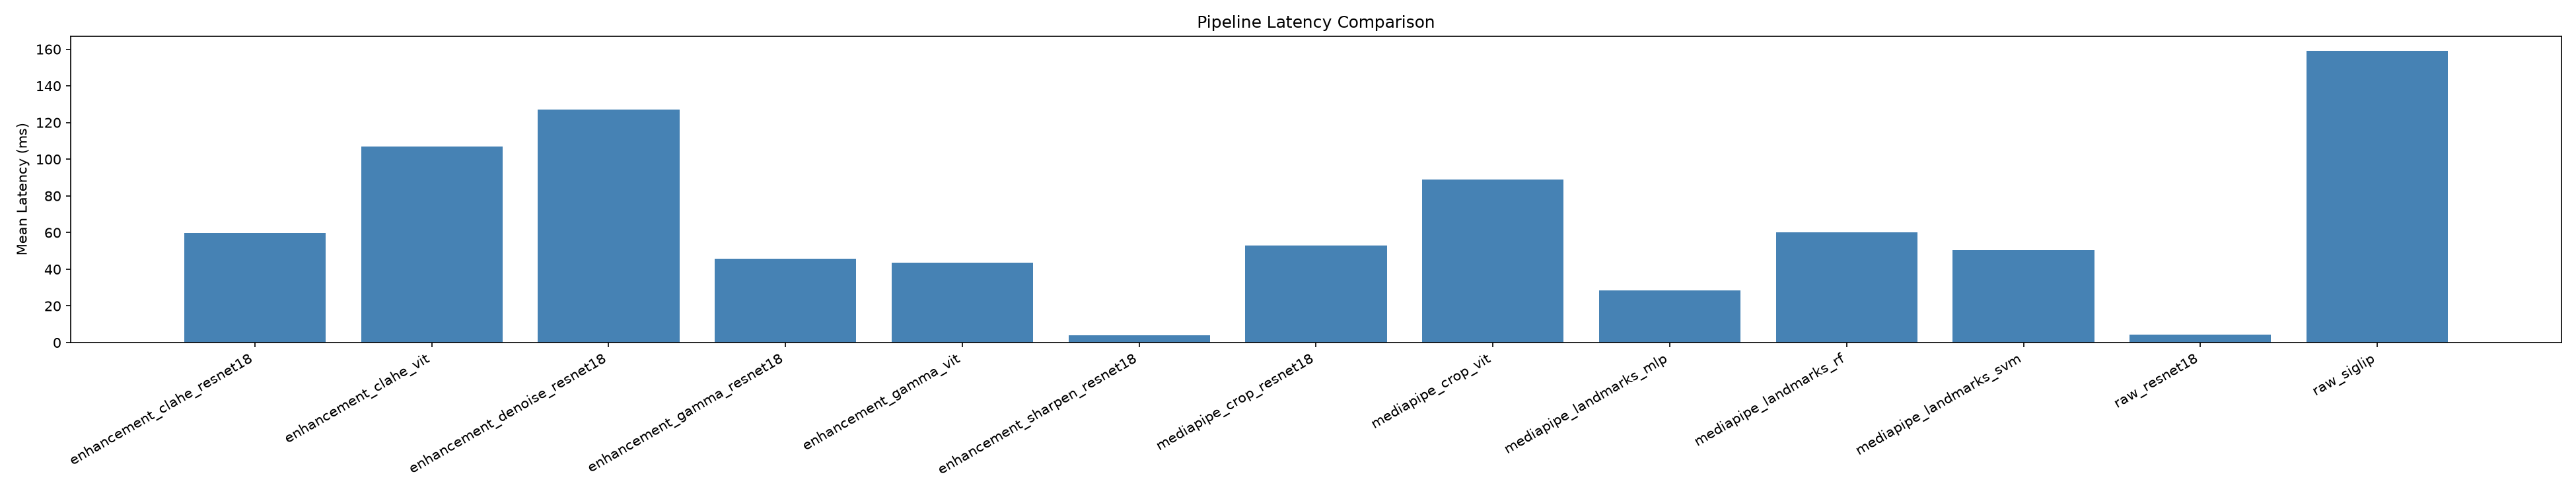
\includegraphics[width=0.78\textwidth]{pipeline_latency_comparison.png}
  \caption{Latency / FPS trade-off. Landmark-based and raw-ResNet-18 pipelines
    reach the highest throughput, making the accuracy--robustness--speed
    trade-off (rather than accuracy alone) the right way to choose a pipeline
    for a given deployment target.}
  \label{fig:latency_chart}
\end{figure}

\begin{figure}[H]
  \centering
  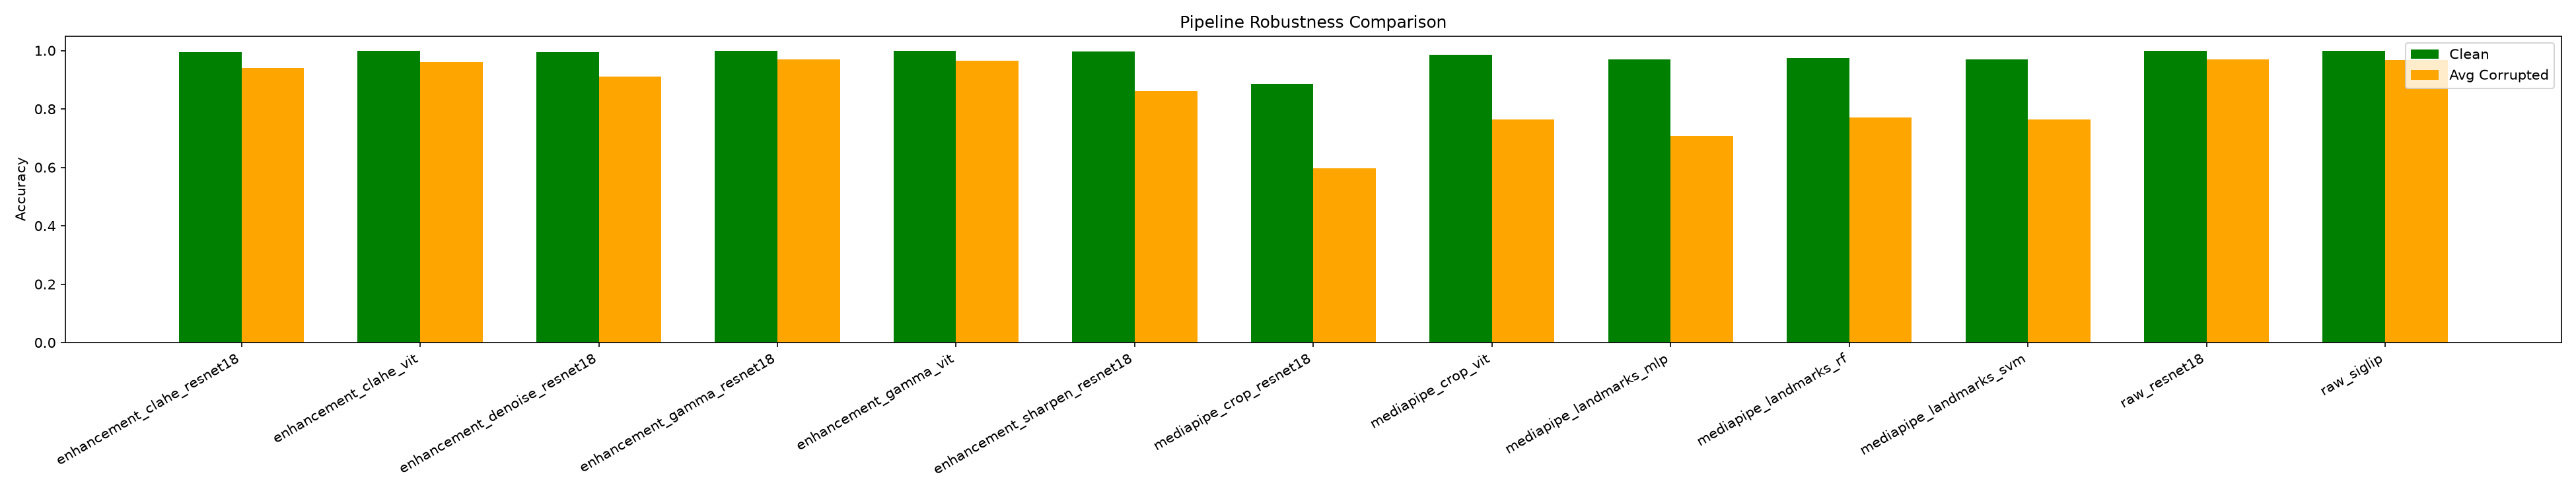
\includegraphics[width=0.85\textwidth]{pipeline_robustness_comparison.png}
  \caption{Accuracy under each of the eight corruption types, per pipeline.
    The MediaPipe-based pipelines are the only ones that reach zero accuracy
    on any corruption type.}
  \label{fig:robustness_chart}
\end{figure}

%% ═══════════════════════════════════════════════════════════════════════════
\section{Qualitative Results}

\subsection{Step-by-Step Pipeline Behavior}

Figure~\ref{fig:recognizer_grid} extends Figure~\ref{fig:repr_grid} to full
pipelines: the same five images are passed through all 13 pipelines, and each
prediction is marked correct (green) or incorrect (red).

\begin{figure}[H]
  \centering
  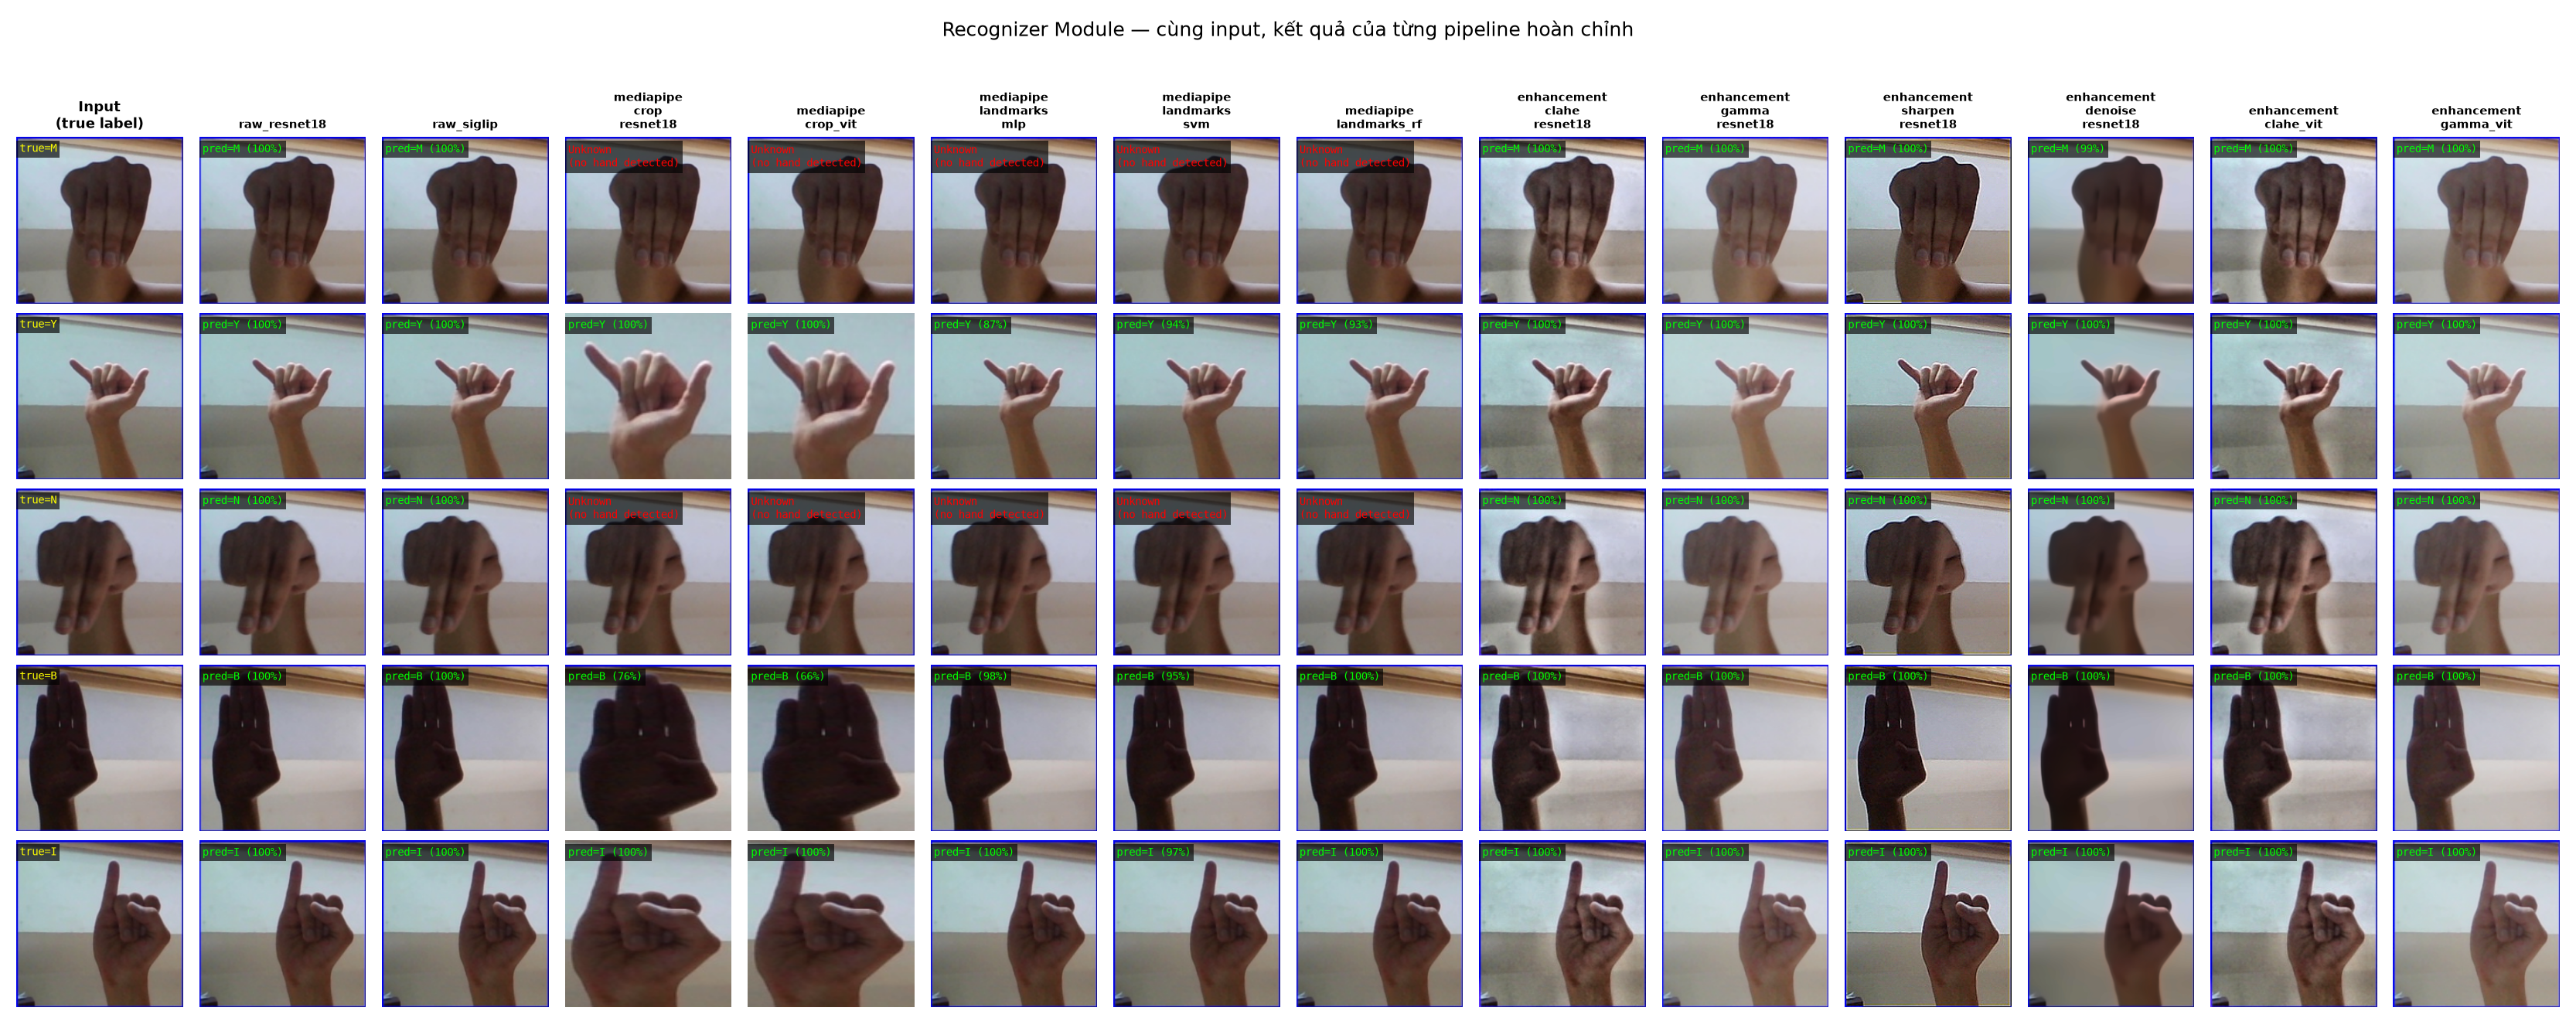
\includegraphics[width=0.97\textwidth]{grid_recognizer.png}
  \caption{Predictions of all 13 pipelines on the same five test images. Every
    MediaPipe-based pipeline (columns sharing the MediaPipe representation) is
    wrong on the exact same rows --- the failure originates once in the shared
    representation stage and propagates identically to every recognizer
    attached to it.}
  \label{fig:recognizer_grid}
\end{figure}

\subsection{Looking Inside the CNN: Grad-CAM}

To confirm that the ResNet-18 classifier itself is not the source of failure,
Figure~\ref{fig:gradcam} visualizes Grad-CAM activations at \codepath{layer4}
for two pipelines that share the same recognizer weights but differ in
representation.

\begin{figure}[H]
  \centering
  \begin{subfigure}{0.95\textwidth}
    \centering
    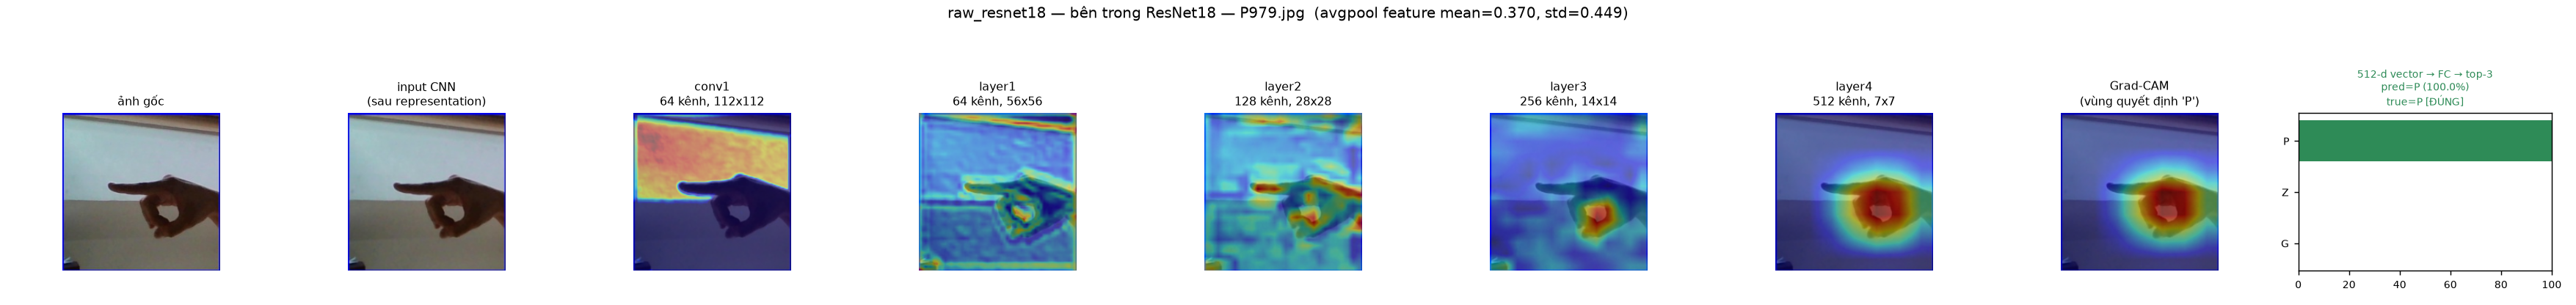
\includegraphics[width=\linewidth]{cnn_internals_raw_resnet18_P979.png}
    \caption{\codepath{raw\_resnet18}: activation maps shrink from $224^2$
      (conv1) to $7^2$ (layer4) while channel count grows $64\rightarrow512$;
      Grad-CAM correctly highlights the hand region.}
  \end{subfigure}
  \vspace{4pt}
  \begin{subfigure}{0.95\textwidth}
    \centering
    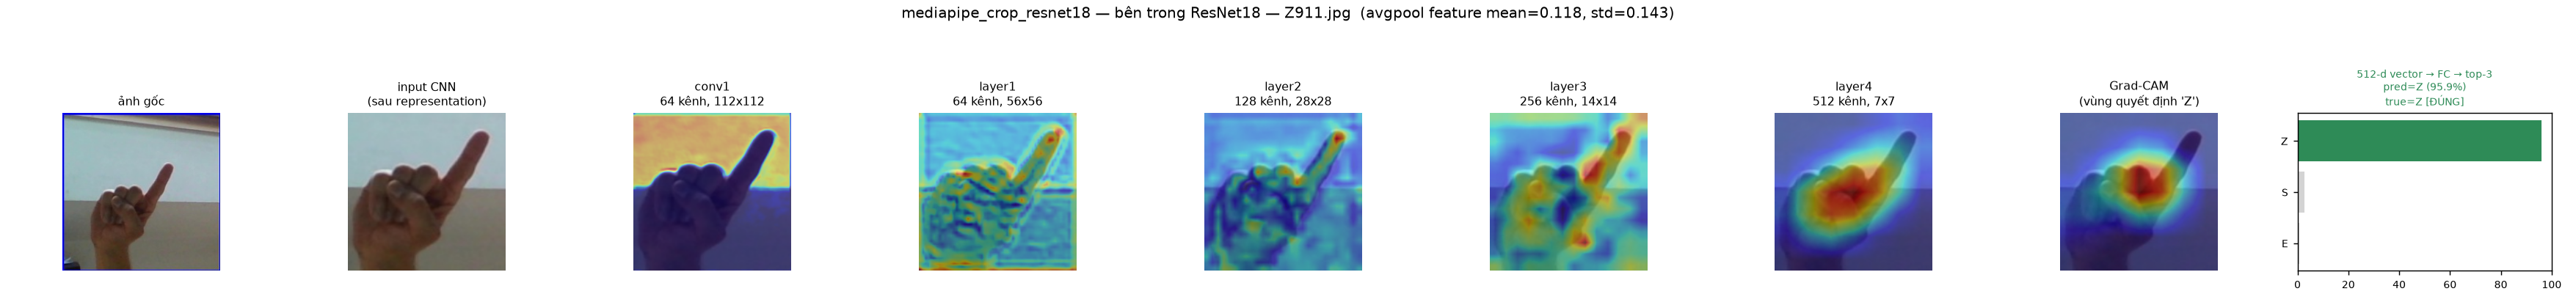
\includegraphics[width=\linewidth]{cnn_internals_mediapipe_crop_resnet18_Z911.png}
    \caption{\codepath{mediapipe\_crop\_resnet18}: same backbone, cropped
      input; Grad-CAM again correctly attends to the hand.}
  \end{subfigure}
  \caption{Grad-CAM at the final convolutional block for two pipelines sharing
    ResNet-18 weights. In both cases the classifier attends to the correct
    region --- confirming that classification failures observed elsewhere in
    this report originate in the upstream representation stage, not in the
    CNN itself.}
  \label{fig:gradcam}
\end{figure}

\subsection{Feature-Space Analysis}

Figure~\ref{fig:embedding_cnn} confirms that ResNet-18's learned 512-d feature
space separates classes just as cleanly as the raw 42-d landmark space
(Figure~\ref{fig:embedding_landmarks}), reinforcing that classification itself
is not the bottleneck for any pipeline studied. Figure~\ref{fig:repr_shift}
then asks a different question: does \emph{changing the representation}
(rather than the class) move a fixed image's feature vector?

\begin{figure}[H]
  \centering
  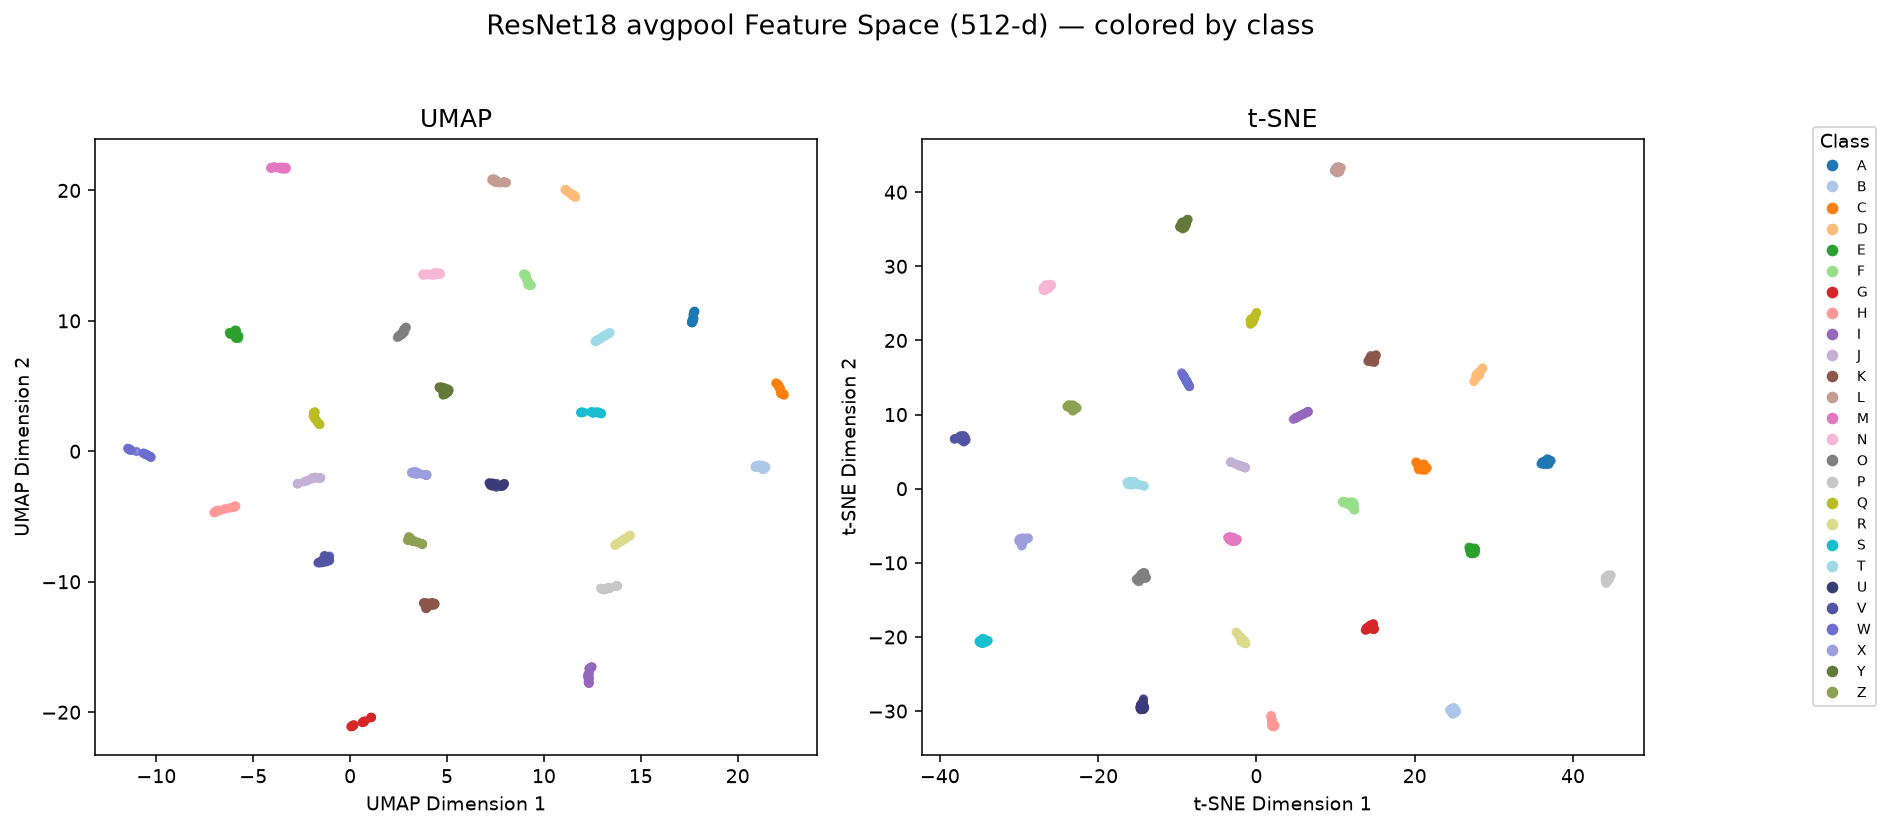
\includegraphics[width=0.62\textwidth]{embedding_cnn_by_class.png}
  \caption{UMAP/t-SNE of 512-d ResNet-18 \codepath{avgpool} embeddings (30
    images/class). Classes separate as cleanly as in landmark space
    (Figure~\ref{fig:embedding_landmarks}).}
  \label{fig:embedding_cnn}
\end{figure}

\begin{figure}[H]
  \centering
  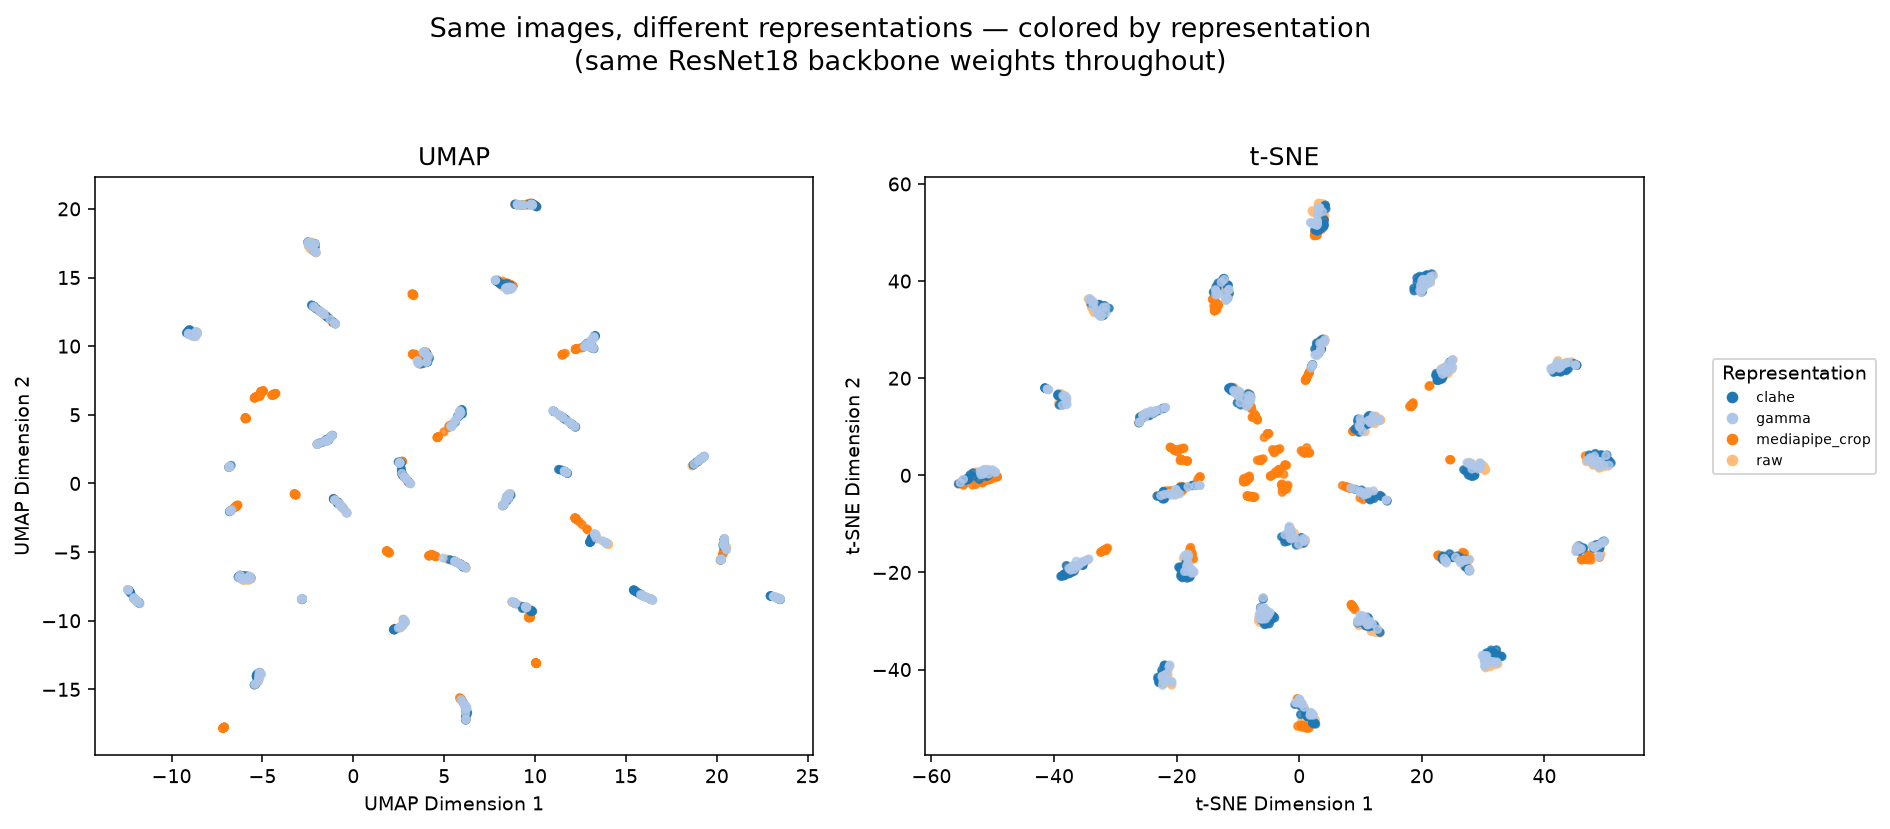
\includegraphics[width=0.68\textwidth]{embedding_representation_shift.png}
  \caption{Same images, four representations (Raw, MediaPipe Crop, CLAHE,
    Gamma), embedded through the same ResNet-18 backbone and colored by
    representation. Raw/CLAHE/Gamma cluster together per image --- mild
    photometric enhancement barely moves the feature vector --- while
    MediaPipe Crop (orange) lands in a visibly different region: changing the
    \emph{representation}, not just lightly enhancing the same image, is what
    actually shifts the feature space the recognizer operates in.}
  \label{fig:repr_shift}
\end{figure}

%% ═══════════════════════════════════════════════════════════════════════════
\section{Case Study: High Reported Accuracy, Yet the System Still Fails}
\label{sec:case_study}

This section makes the abstract metric pitfall of Section~\ref{sec:metrics}
concrete using \codepath{mediapipe\_crop\_vit} --- a pipeline that combines
MediaPipe hand-cropping with the strongest recognizer in this study, a
pretrained SigLIP ViT.

\begin{figure}[H]
  \centering
  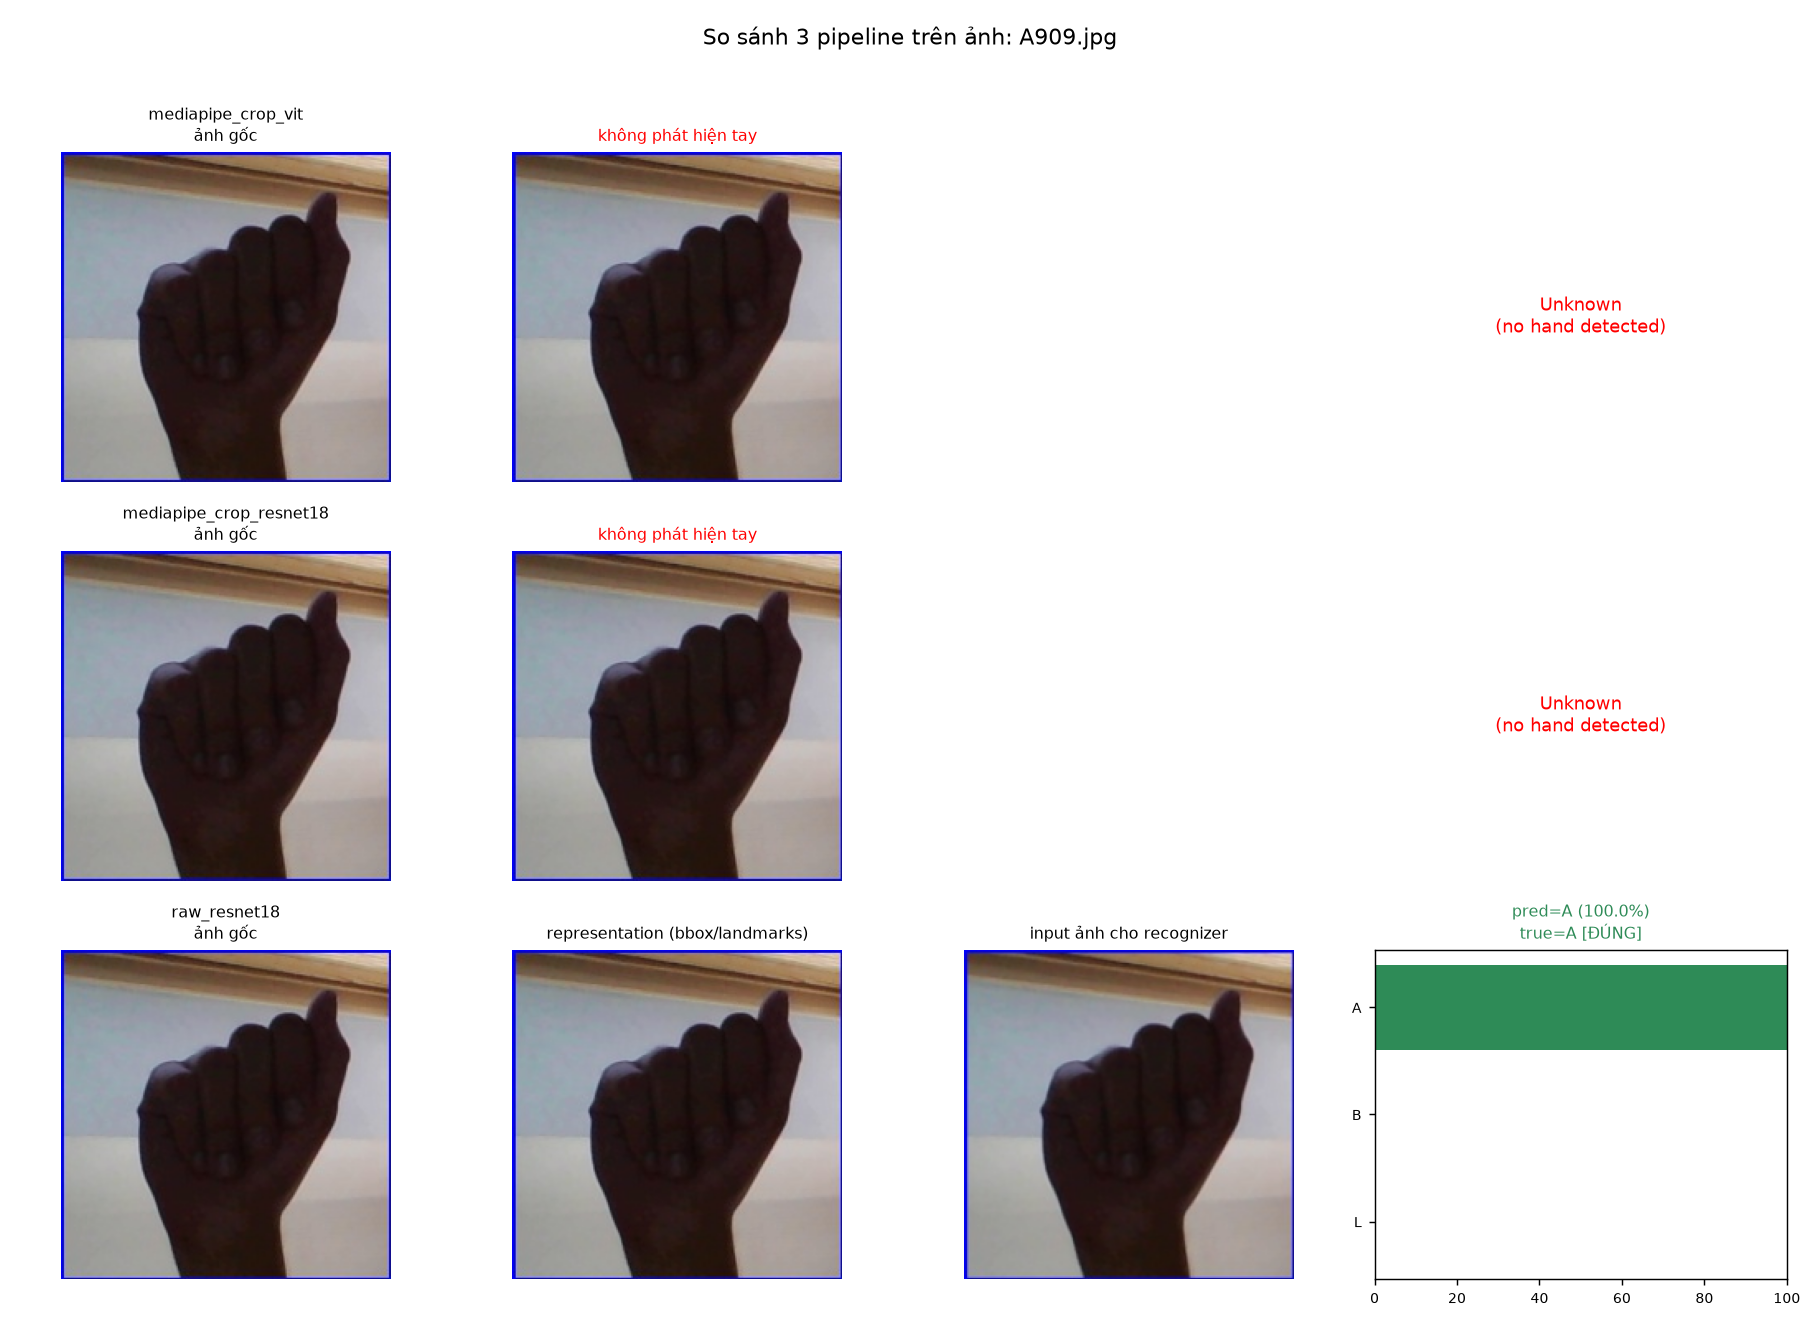
\includegraphics[width=0.55\textwidth]{compare_A909_hand_not_detected.png}
  \caption{The same low-contrast test image, run through three pipelines.
    \codepath{mediapipe\_crop\_vit} and \codepath{mediapipe\_crop\_resnet18}
    both output \textsc{Unknown} --- the upstream hand detector failed before
    either recognizer had a chance to classify anything. \codepath{raw\_resnet18},
    which has no detection stage, correctly predicts ``A'' with 100\%
    confidence on the identical pixels.}
  \label{fig:case_study}
\end{figure}

Applying Eq.~\eqref{eq:clean_acc}, \codepath{mediapipe\_crop\_vit} reports a
clean accuracy of 98.5\%, the best result among MediaPipe-based pipelines
(Table~\ref{tab:summary_results}). But this number is computed only over the
$N - HDFR\cdot N \approx 2{,}142$ images on which a hand was detected.
Applying Eq.~\eqref{eq:real_acc} over the full 2{,}600-image test set:
\begin{equation}
  \text{real\_accuracy}(\text{mediapipe\_crop\_vit}) =
  \frac{2110}{2600} = 81.15\%,
\end{equation}
a gap of \textbf{17.4 percentage points} below the reported figure. The
recognizer itself is not at fault --- as Figure~\ref{fig:gradcam} confirms,
the classifier correctly attends to hand regions when it receives them; the
gap exists purely because 17.15\% of inputs never reach the classifier at
all, and the standard accuracy formula does not count that as failure. The
practical conclusion is unambiguous: a two-stage pipeline's reliability is
upper-bounded by its weakest stage, and that bound is invisible unless
accuracy is computed over \emph{all} inputs, not only the ones a detector
chose to act on.

%% ═══════════════════════════════════════════════════════════════════════════
\section{Discussion}

Three findings, taken together, answer the question posed in
Section~\ref{sec:motivation}. First, hand-cropping and landmark extraction do
not improve the recognizer's job in this dataset --- Figure~\ref{fig:embedding_landmarks}
shows the classes are already linearly separable from raw landmarks, and
Figure~\ref{fig:embedding_cnn} shows ResNet-18 separates them just as well
from raw pixels, so there is no classification difficulty for a smarter
representation to solve. Second, the representation stage introduces a new
failure mode (missed hand detection) that the recognizer cannot recover from,
and this failure mode is invisible in the standard accuracy metric
(Section~\ref{sec:case_study}). Third, the failure compounds catastrophically,
not gracefully, under corruption (Figure~\ref{fig:robustness_chart}): rather
than a modest accuracy drop, MediaPipe-based pipelines reach exactly 0\%
accuracy on at least one corruption type, because a single brittle upstream
stage gates the entire pipeline.

The practical implication for system design is that architectural simplicity
should be the default, not the fallback: a raw-image or lightly-enhanced
representation fed directly to a single classifier is both more accurate end
to end and structurally immune to this class of failure, since there is no
detection stage to fail in the first place.

%% ═══════════════════════════════════════════════════════════════════════════
\section{Limitations}

Several representation modules described in the project's design
(YOLO-based cropping, segmentation-mask cropping, and RGB+landmark fusion)
remain unimplemented stubs and are not part of the 13 evaluated pipelines.
All results are reported on a single dataset (ASL Alphabet, studio-lit,
relatively clean backgrounds); the absolute hand-detection failure rate and
the size of the accuracy gap in Section~\ref{sec:case_study} would likely be
different, and plausibly larger, on uncontrolled real-world webcam footage.
The SigLIP ViT recognizer is used as a third-party pretrained model without
further fine-tuning on this dataset, so its reported numbers reflect transfer
performance rather than a fully optimized model.

%% ═══════════════════════════════════════════════════════════════════════════
\section{Conclusion}

We built a modular framework that separates the representation and recognizer
stages of a static ASL alphabet recognition system, and used it to evaluate 13
pipelines under one shared protocol covering clean accuracy, robustness, and
a previously-hidden accuracy pitfall. The results show that adding a hand
detector does not improve recognition in this setting: it does not make
classification easier (the classes are already separable without it), and it
introduces a brittle stage that silently removes 17\% of inputs from the
standard accuracy calculation while contributing zero accuracy under several
corruption types. The simplest pipelines studied --- a raw or lightly enhanced
image fed directly to a single recognizer --- are simultaneously the most
accurate end to end and the most robust, directly answering the motivating
question of this report: a smarter-looking representation is not automatically
a better one, and verifying that claim requires evaluating the full pipeline
under metrics that cannot hide its failures.

%% ═══════════════════════════════════════════════════════════════════════════
\section{References}

\begin{thebibliography}{9}

\bibitem{mediapipe}
C.\ Lugaresi et al.,
``MediaPipe: A Framework for Building Perception Pipelines,''
\textit{arXiv:1906.08172}, 2019.

\bibitem{resnet}
K.\ He, X.\ Zhang, S.\ Ren, and J.\ Sun,
``Deep Residual Learning for Image Recognition,''
\textit{IEEE Conf.\ on Computer Vision and Pattern Recognition (CVPR)}, 2016.

\bibitem{siglip}
X.\ Zhai, B.\ Mustafa, A.\ Kolesnikov, and L.\ Beyer,
``Sigmoid Loss for Language Image Pre-Training,''
\textit{IEEE Int.\ Conf.\ on Computer Vision (ICCV)}, 2023.

\bibitem{aslalphabet}
Kaggle,
``ASL Alphabet Dataset,''
\url{https://www.kaggle.com/datasets/grassknoted/asl-alphabet}.

\bibitem{umap}
L.\ McInnes, J.\ Healy, and J.\ Melville,
``UMAP: Uniform Manifold Approximation and Projection for Dimension Reduction,''
\textit{arXiv:1802.03426}, 2018.

\bibitem{tsne}
L.\ van der Maaten and G.\ Hinton,
``Visualizing Data using t-SNE,''
\textit{Journal of Machine Learning Research}, 2008.

\bibitem{gradcam}
R.\ R.\ Selvaraju et al.,
``Grad-CAM: Visual Explanations from Deep Networks via Gradient-based Localization,''
\textit{IEEE Int.\ Conf.\ on Computer Vision (ICCV)}, 2017.

\end{thebibliography}

\end{document}
